\documentclass{beamer}
\usepackage[backend=bibtex, citestyle=authoryear]{biblatex}
\addbibresource{dataset_references.bib}
\usepackage{graphicx}
\usetheme{default}

\title{How the Makusafe data set is different}
\subtitle{why we shouldn't expect common fall detection schemes to work on Makusafe data}
\author{Alden Bradford}
\institute{Purdue University / The Data Mine}
\date{\today}

\begin{document}

\begin{frame}
\titlepage
\end{frame}

\begin{frame}{Other fall detection schemes}
We have based a lot of our strategy on two recent papers, both of which study fall detection using only accelerometer data.
\begin{itemize}
\item (\cite{althobaiti2020triaxial}) provides a helpful literature review, describing various strategies people have used for fall detection and the degree of success they had. The article is mainly a description of an experiment where research participants performed motions in a controlled environment, and researchers attempted to build a fall detection strategy based on the measured data.
\item (\cite{vseketa2021event}) focuses on using a data segment (window) centered around a high peak acceleration, and seeks to find a good choice of window size.
\end{itemize}
\end{frame}

\begin{frame}{Our goal here}
These papers both had the goal of differentiating between hazardous movements (mainly falls) and nonhazardous movements called "activities of dailiy living" (ADL). Both reported high F-scores (over 95\%), which is a combined measure of positive and negative predictive value. Most of the features we implemented were suggested by these two papers.

So far, our attempts to classify the makusafe data (\cite{makusafe}) have been able to get F-scores of only around 20\%. In order to understand this discrepancy, we set about trying to reproduce the methods used in (\cite{vseketa2021event}), to see if we can figure out why we have not seen the same success.
\end{frame}

\begin{frame}{Other data sets}
In (\cite{vseketa2021event}), the authors rely on three publicly available datasets:
\begin{description}
\item[FallAllD] (\cite{bnya-mn34-20})
\item[SisFall] (\cite{sucerquia2017sisfall})
\item[Erciyes] (\cite{ozdemir2014detecting})
\end{description}
The FallAllD and SisFall datasets both have records with significantly higher sample rates than (\cite{makusafe}). To ensure a fair comparison, we used Fourier analysis to resample all data sets to 25 Hz. The Erciyes dataset was already sampled at 25 Hz.

Following the method in (\cite{vseketa2021event}) we found all peaks higher than a given threshold (different for each set) and extracted an 8-second window centered around each peak. This gave us several thousand samples, labeled by their motions.
\end{frame}

\begin{frame}{Exploration through factor analysis}
For each sample, we computed all the features recommended in (\cite{vseketa2021event}).

By using factor analysis, we were able to select ten features which explain most of the variance in the feature space.

\begin{figure}[h!]
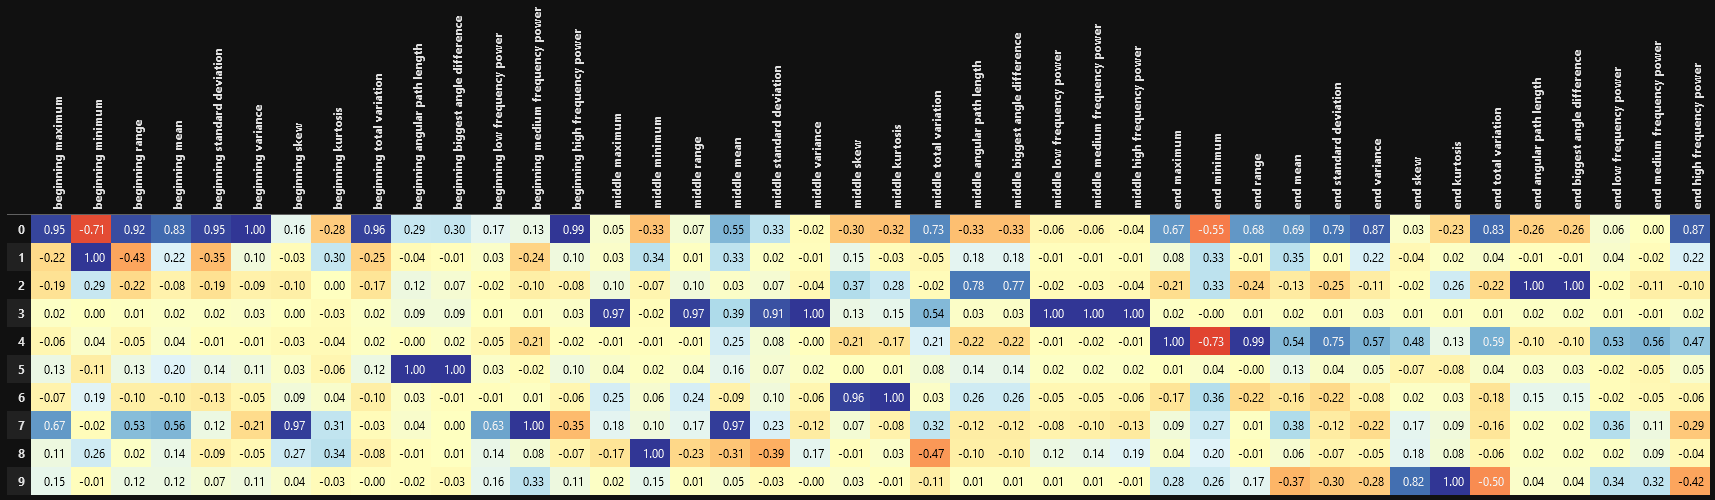
\includegraphics[width=\textwidth]{factors}
\end{figure}
\end{frame}

\begin{frame}{Feature scatter plot}
Each point is an incident, and its color is a motion.
\begin{figure}
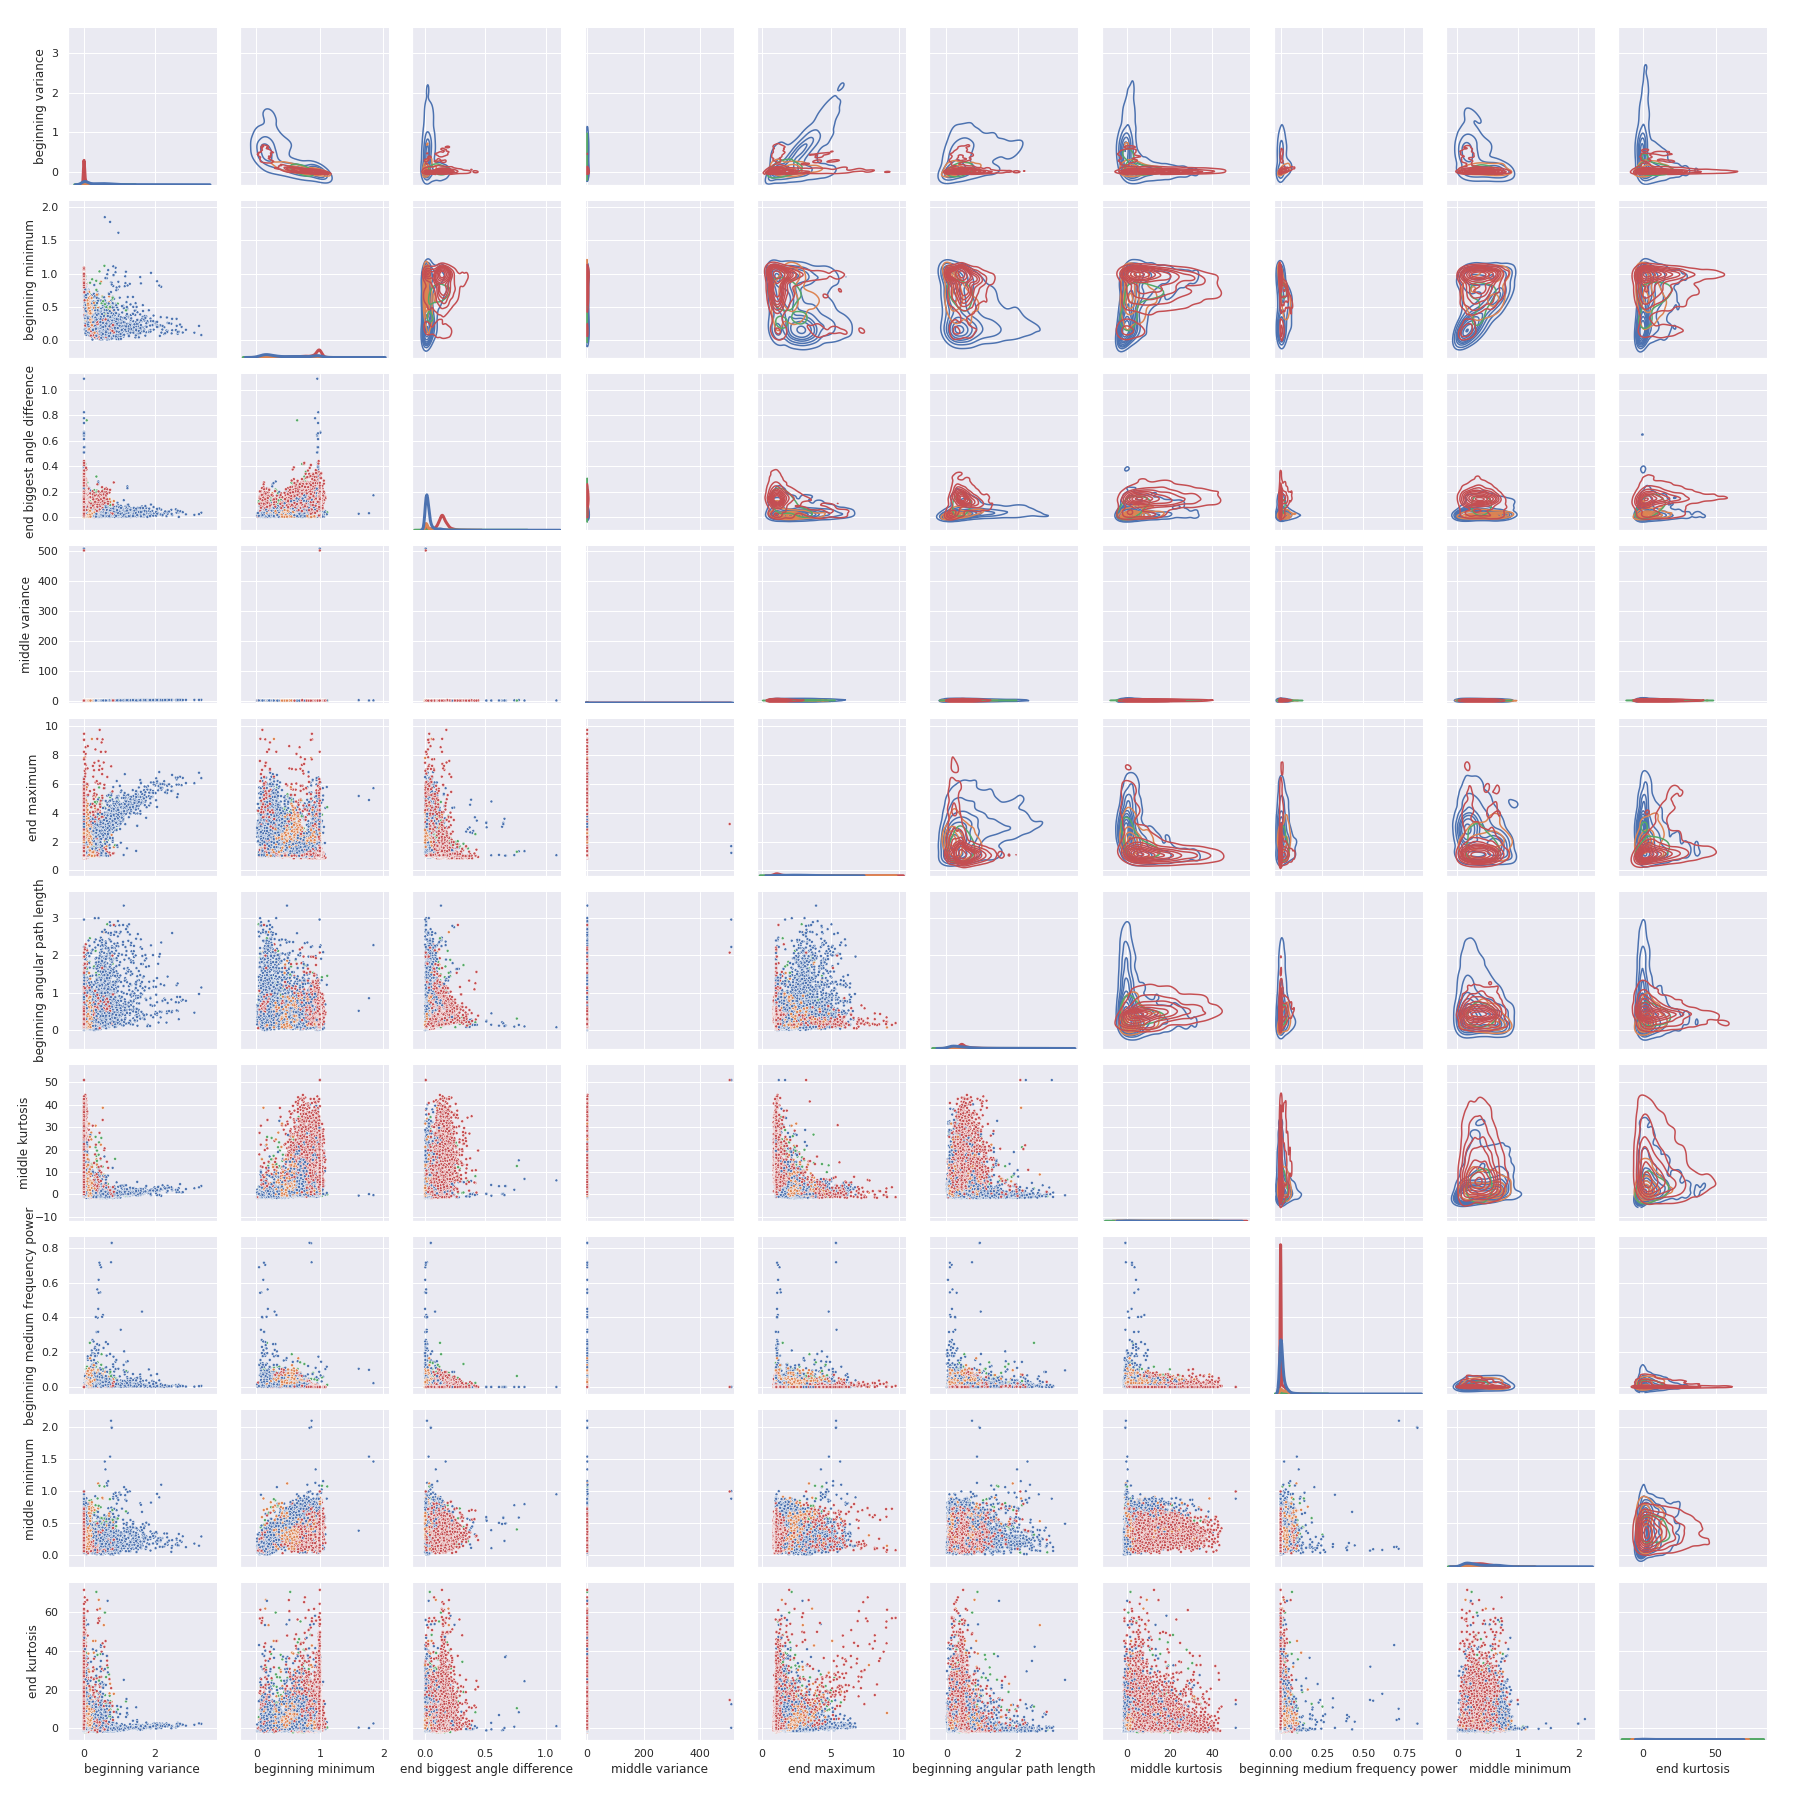
\includegraphics[height=0.8\textheight]{pair_plot_othersets}
\end{figure}
\end{frame}

\begin{frame}{One of those plots caught our eye}
\begin{figure}
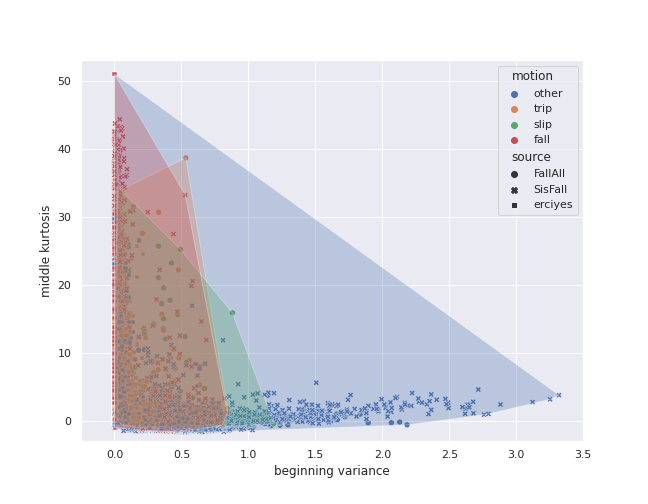
\includegraphics[height=0.6\textheight]{variance_vs_kurtosis_other_datasets}
\end{figure}
Notice that most of the points with a high variance at the beginning of the sample are ADL, while most of the samples with high kurtosis in the middle are falls.
\end{frame}

\begin{frame}{Kurtosis, Variance}
\begin{description}
\item[Variance] at the beginning measures how much movement was happening before the incident. It makes sense that a lot of motion would increase the chance of a false alarm.
\item[Kurtosis] in this case measures how big the central peak was, compared to the typical variation of the sample. It makes sense that a large peak would correspond to a hazardous motion.
\end{description}
\end{frame}


\begin{frame}{Just the FallAllD data}
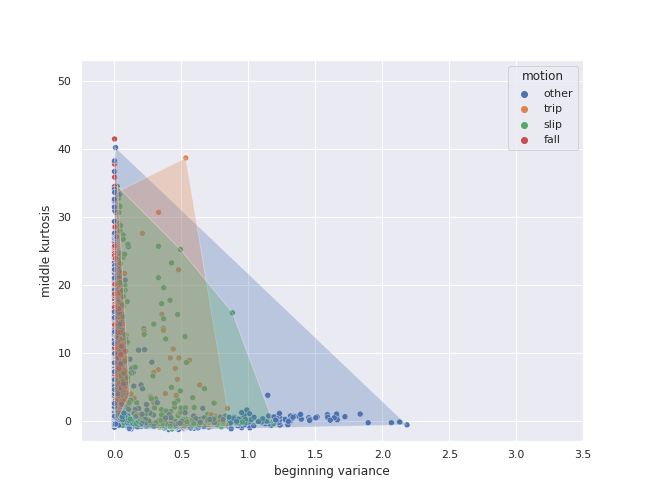
\includegraphics[height=\textheight]{variance_vs_kurtosis_FallAll}
\end{frame}


\begin{frame}{Just the SisFall data}
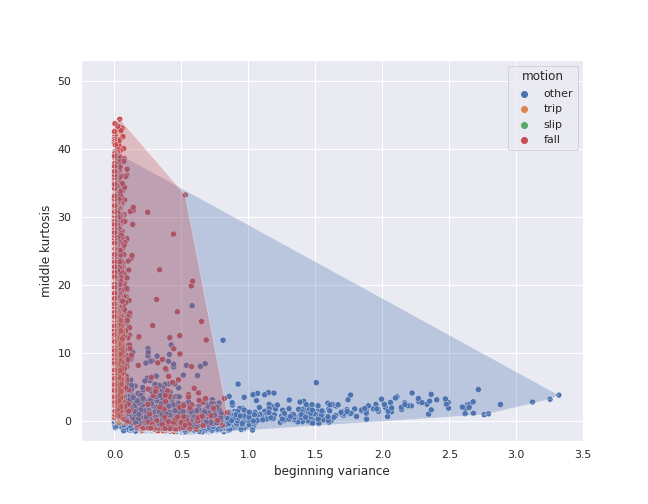
\includegraphics[height=\textheight]{variance_vs_kurtosis_SisFall}
\end{frame}

\begin{frame}{Just the Erciyes data}
\includegraphics[height=\textheight]{variance_vs_kurtosis_Erciyes}
\end{frame}


\begin{frame}{How does makusafe compare?}
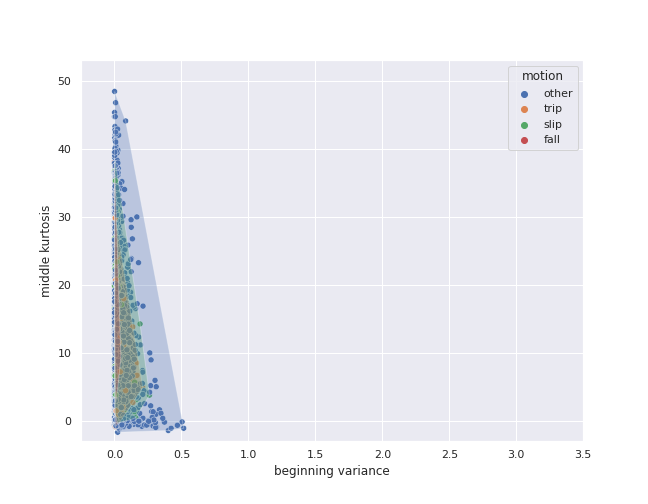
\includegraphics[height=\textheight]{variance_vs_kurtosis_makusafe}
\end{frame}


\begin{frame}{Conclusions}
\begin{itemize}
\item There is something different about the Makusafe data, something not explained by differences in sampling rate, different trigger thresholds, different mounting locations, or a lack of gyroscope.
\item The hazards are almost trivially easy to separate in the other data sets, using the given features.
\item We should not expect to be able to use the same strategy on the Makusafe data.
\end{itemize}
\end{frame}

\begin{frame}{Potential causes}
\begin{description}
\item[real versus simulated] The other data sets are using simulated falls in a controlled environment. This type of motion may be significantly different from a real fall.
\item[range of activities] Since most sources are interested in fall detection among the elderly, they consider only ADLs which the elderly are likely to perform. The activities Makusafe customers engage in may not be well-covered by those types of non-hazardous activity.
\item[differences in definition] It could be that there are incidents in the Makusafe set which would be classified as a fall by the standards of these other papers, but which Makusafe customers would not consider worth reporting.
\end{description}
\end{frame}


\begin{frame}{Future directions}
\begin{itemize}
\item We should not expect to be able to apply strategies from other papers to our data.
\item We should reconsider our choice of features -- look for a pattern which applies specifically to Makusafe data.
\item We should reconsider what we want our goal to be. It may be unreasonable to think we can find a classifyer with a high positive predictive value. Some alternatives are:
\begin{itemize}
	\item find a classifyer with a high negative predictive value. Even if we can't pick out the hazards, we may be able to remove the bulk of the non-hazards.
	\item Build an aggregate index of risk -- something which can predict what fraction of incidents matching a given profile will be classified as hazards. This could be used to identify dangerous patterns without necessarily being able to identify dangerous incidents.
\end{itemize}
\end{itemize}
\end{frame}

\begin{frame}[allowframebreaks]{References}
\printbibliography
\end{frame}

\end{document}